%###############################################
%# RTUPB
%###############################################
\subsection{Données pré et post opératoires RTUPB}

RTUPB est une table composée de 36 patients. 
	
\begin{figure}[!h]
\centering
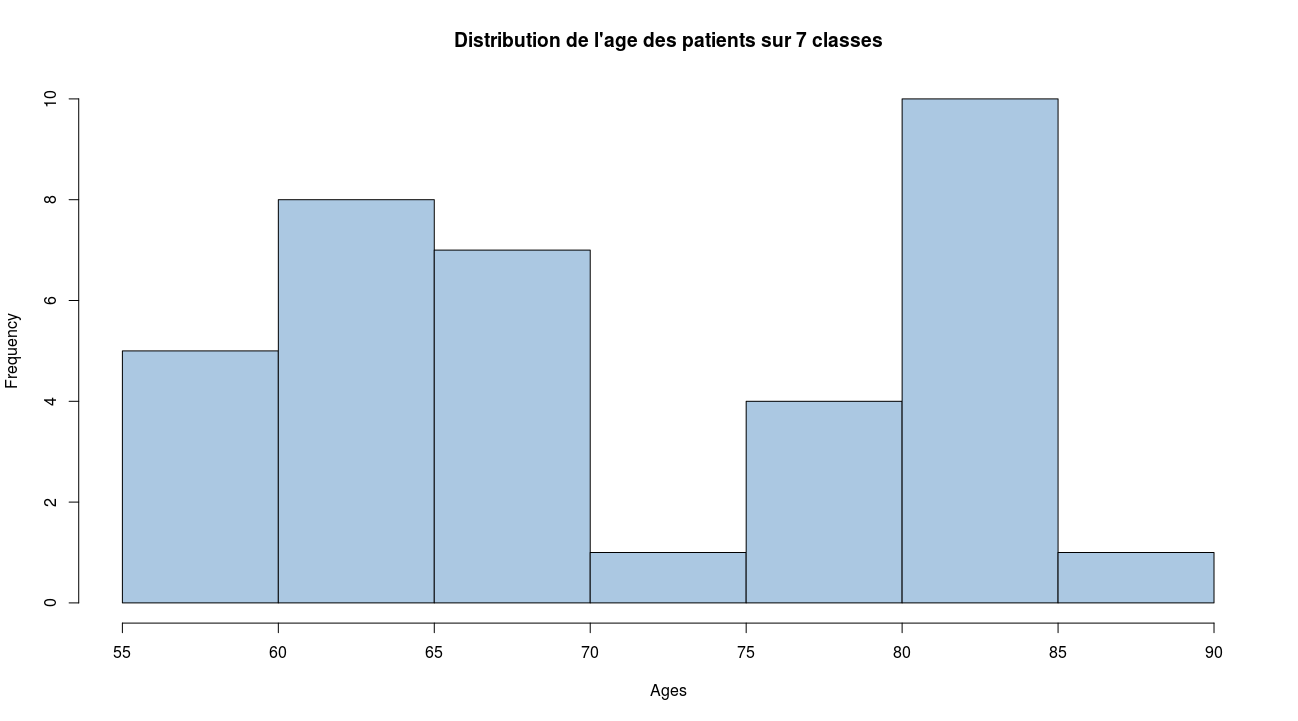
\includegraphics[width=0.75\textwidth]{../Fig/RTUPB/rtupb-age-frequency.png}
\caption{Distribution des patients suivant l'age.}
\end{figure}

Dans les analyses suivantes nous omettrons les dimensions suivantes  (invariantes)  :  
\begin{itemize}
\item Technique
\item Evenement H.D
\item Transfusion PerO
\item reprise au bloc 
\end{itemize}


\subsubsection{Mise en evidence des corrélations}

Le corrélogramme suivant montre une vision synthétique des relations  entre les variables.

\begin{figure}[!h]
\centering
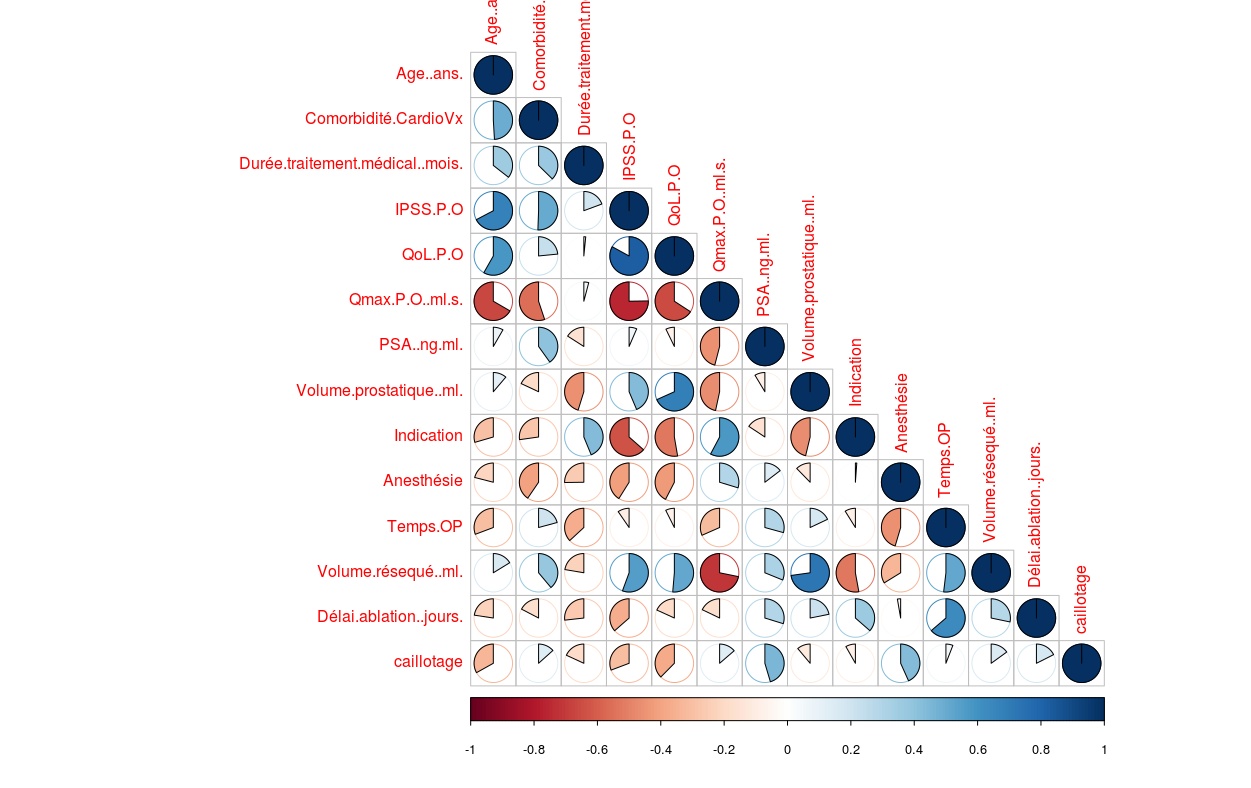
\includegraphics[width=0.75\textwidth]{../Fig/RTUPB/rtupb-matrice-cor-graph.png}
\caption{corrélogramme RTUPB.}
\end{figure}

Les variables  \emph{IPSS P.O} et   \emph{QoL P.O}  semblent être corrélées ce qui peut sembler logique à la connaissance du fait 
qu’elles représentent pour l’une un indicateur de gène et pour l’autre un indicateur une qualité de vie post opératoire.De même  pour les variables Volume prostatique et Volume resequé . Aussi nous avons une corrélation \textbf{negative} interressante entre le IPSS P.O et le QMAX PO (ml/s) (plus le patient à un QMax elevé moins il semble géné
\newpage 

\subsubsection{Distribution des variables Post op. 18 mois}

\begin{figure}[!h]
\centering
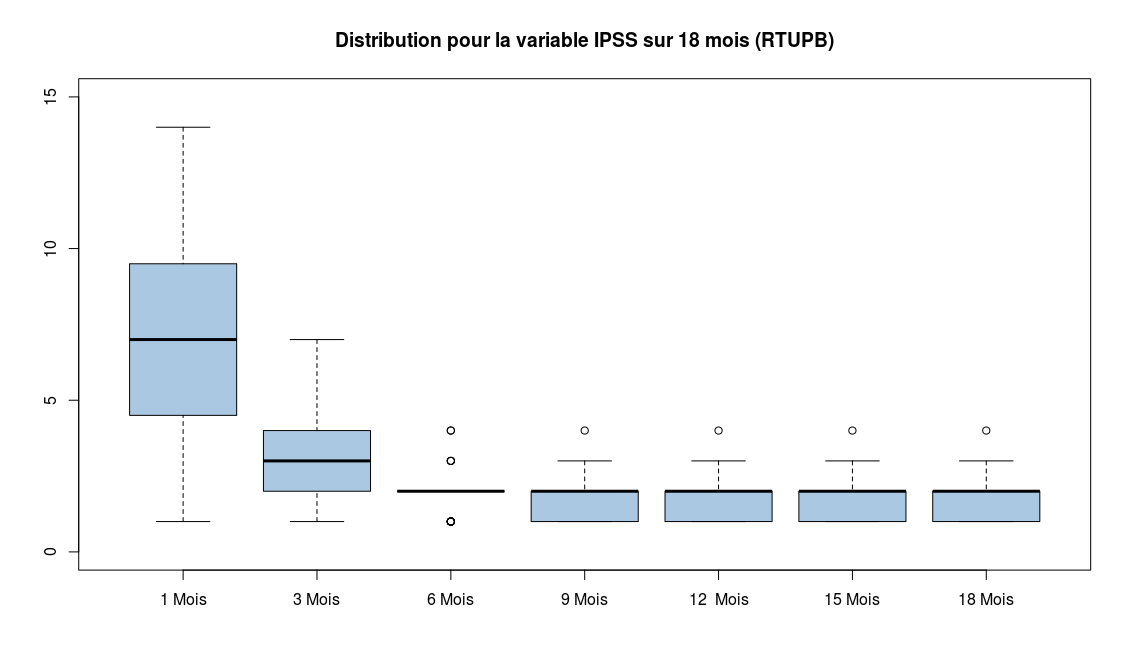
\includegraphics[width=0.75\textwidth]{../Fig/RTUPB//rtupb-boxplot-post-ipss}
\caption{distribution IPSS 18 mois}
\end{figure}


\begin{figure}[!h]
\centering
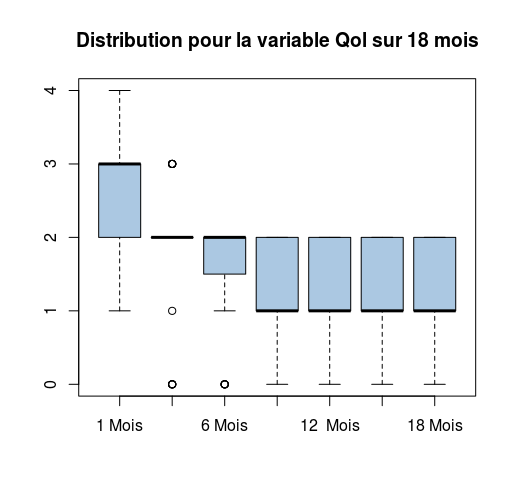
\includegraphics[width=0.75\textwidth]{../Fig/RTUPB//rtupb-boxplot-post-Qol}
\caption{distribution Qol 18 mois}
\end{figure}

\begin{figure}[!h]
\centering
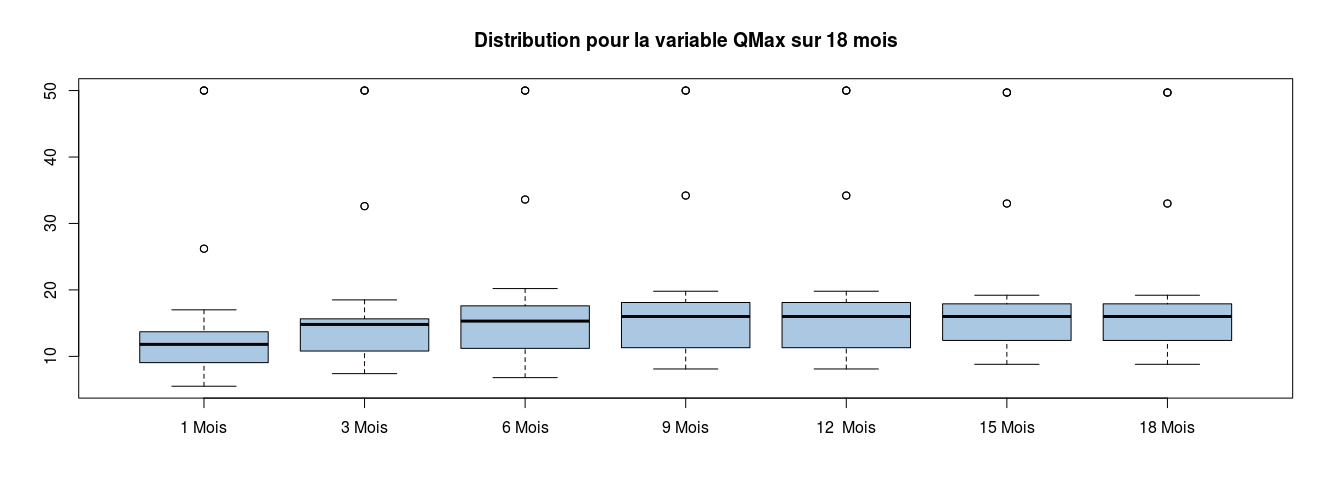
\includegraphics[width=0.80\textwidth]{../Fig/RTUPB//rtupb-boxplot-post-Qmax}
\caption{distribution Qmax 18 mois}
\end{figure}






\newpage

%###############################################
%# VPPBS
%###############################################
\subsection{Données pré et post opératoires VPPBS }
\newpage


%###############################################
%# VAPOR
%###############################################
\subsection{Données pré et post opératoires VAPOR}
\newpage